\chapter{Introduction}
\label{cha:intro}

\begin{figure}[thb!]
	\centering
	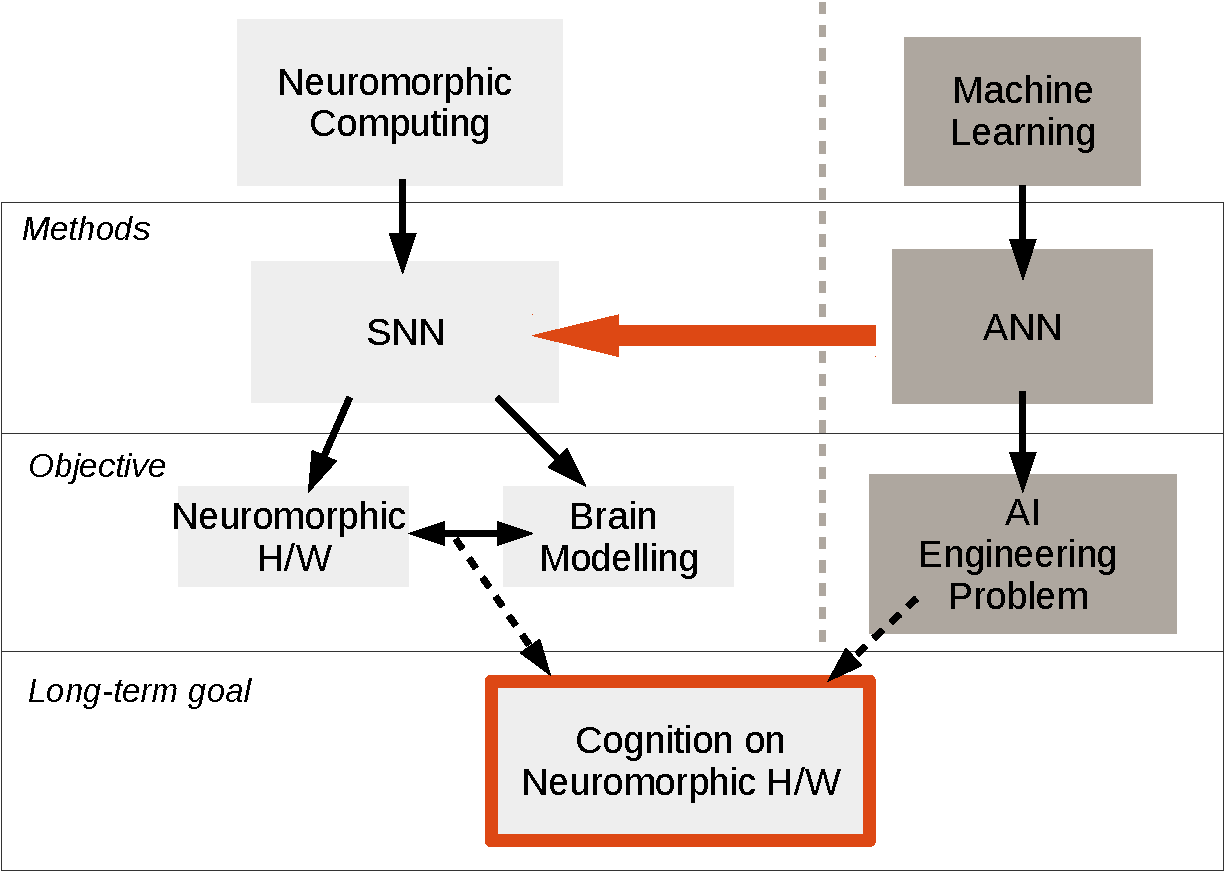
\includegraphics[width=0.8\textwidth]{pics_intro/intro1.pdf}
	\caption{The story line of the thesis.}
	\label{fig:intro}
\end{figure}

%Problem, motivation and significance
%TODO the origin of neuromorphic computing
Promising advances in computing power and machine learning have empowered computers with a rapid growing performance on more and more cognitive tasks, such as recognising objects and playing GO. However, this beat-human performance is supported by huge amount (for example 1~MW on AlphaGO~\cite{silver2016mastering}) of energy use comparing to an average human brain, 20~W.
The impressive disparities of several magnitude in energy consumption drives the research into biologically-inspired computer design.
With the widespread introduction over the last half cen
tury of the stored-programme computer into all areas of
human activity we have an alternative information processing
paradigm against which the brain may be compared, yet
despite superficial similarities in their roles as information
processing and control systems, it is clear that the principles
of operation of the brain and the computer are very different.
While computers excel at speed and precision, the brain still
wins in coping with novelty, complexity and ambiguity, and
in practical tasks such as facial recognition and controlling
bipedal locomotion.

Rather than using Boolean logic, precise digital rep-
resentations, and clocked operations, nervous systems carry
out robust and reliable computation using hybrid analog/
digital unreliable components; they emphasize distributed,
event-driven, collective, and massively parallel mecha-
nisms, and make extensive use of adaptation, self-
organization, and learning.

This difference in capabilities has encouraged computer
engineers from the earliest days of computing to wonder
whether there might not be different principles at work in the
brain that could profitably be applied in the design of
machines. Where these principles are derived from our (par-
tial) understanding of the structure and characteristics of
neurons—the basic components from which the brain is
constructed—and the complex networks of neurons in the
brain, the resulting systems are categorized as neuromorphic
computers. This terminology has come to be applied parti
cularly where the medium in which the system is built is
based upon very large-scale integrated (VLSI) circuits microchips.
Although it is still far from understanding the brain thoroughly, the performance gap is believed to lie in the fundamental computing units and the way they act.
A feature of the biological brain is that while commu
nication uses digital techniques for fast signalling over all but
the shortest distances, all of the processing in neurons and
synapses uses much more efficient analogue chemical tech
niques [3]. This mixed-signal approach contrasts with the all-
digital designs of current general-purpose computers where
digital logic delivers the noise-immunity and deterministic
behaviour that is expected of the universal Turing machine.
Biology sacrifices determinism for efficiency—an approach
that may be of interest to future computer engineers designing
systems, such as robot vision systems, where absolute acc
uracy is in any case unachievable, and energy-efficiency is a
primary requirement.

Neuromorphic engineering (NE) is a research field that
is addressing these issues by designing and fabricating
electronic neural systems whose architecture and design
principles are based on those of biological nervous sys
tems.
The goal of neuromorphic computing is to observe the
formidable complexity of the biological brain and to some
how extract from what is known about its structure and
principles of operation some more abstract principles that can
be applied in a practical engineered system.


%Lee Sedol used about 20 Watts of power to operate. By contrast, AlphaGo runs on a whopping 1920 CPUs and another 280 GPUs for an estimated power consumption of approximately 1 MW (200 W per CPU and 200 W per GPU). That’s 50,000 times as much power as the amount of power that Lee Sedol’s brain uses and the two are not quite evenly matched but it is close enough to use for comparison.

%Simulating the cognitive functions of human intelligence on a machine thus to make it think and act rationally builds up the research field of Artificial Intelligence (AI)~\cite{konar1999artificial}, and has been a major challenge in modern science.
%Despite of the promising progresses in weak AI where computers win some particular intelligent task such as image classification on ImageNet, humans still outperforms the most powerful machines in relatively more complicated tasks, for example vision, in terms of not only capability but also energy efficiency and latency.
%Although it is still far from understanding the brain thoroughly, the performance gap is believed to lie in the fundamental computing units and the way they act. %interact and build up
%Great breakthroughs of machine learning applications in Artificial Neural Network~(ANN) form a successful evidence of connectionism, which uses interconnected networks of simple units to study the brain behaviours.
%To receive further benefits to build energy-efficient machines with cognitive intelligence, neuromorphic computing (or neuromorphic engineering) carries out biologically-plausible neural models instead CPU-like logic and synchronous operations by mimicking the brain.

%TODO Short history with inital aim
Carver Mead proposed in the late 1980s (Mead,1989) and that is known as neuromorphic engineering. Mead’s idea was to use very-large-scale integration (VLSI) technology to build electronic circuits that mimic the architecture of the nervous system.
The term neuromorphic engineering was coined by
Carver Mead in the late 1980s to describe Very Large Scale
Integration (VLSI) systems comprising analog circuits and
built to mimic biological neural cells and architectures
. Since then, NE has been attempting to identify neural
types of computational principles, by implementing bio-
physically realistic models of neural systems in VLSI
technology to reproduce the same physics of computation.
The first electronic devices inspired by this concept were analog circuits that exploited the sub-threshold properties of transistors to emulate the biophysics of real neurons.
Today the term neuromorphic refers to any analog, digital, or hybrid VLSI system whose design principles are inspired by those of biological neural systems (Indiveri et al., 2011).

Neuromorphic engineering combines the architectural and computa
tional principles of systems neuroscience with semiconductor electron
ics, with the aim of building efficient and compact devices that mimic the
synaptic and neural machinery of the brain. The energy consumptions
promised by neuromorphic engineering are extremely low, comparable
to those of the nervous system. Until now, however, the neuromorphic
approach has been restricted to relatively simple circuits and special
ized functions,

The examples cited above, and others not mentioned
here, show the widespread and diverse interest in using
neuromorphic techniques to model biological processes. This
is a two-way process whereby engineers learn principles from
neuroscience to incorporate into their models, and in return
neuroscientists learn from the results those engineers get from
their models. In some cases the goal is very close reproduc-
tion of detailed biological phenomena; in others the goal is to
apply more abstract biological principles to the solution of
engineering problems. All underline the point that there is still
a great deal to learn about, and to learn from, biological
nervous systems, and building models is a great way to learn!

%Problem of memory wall and dark silicon.
The microprocessor/memory performance gap, or the Von Neumann bottleneck, greatly exacerbated in the past decade, which indicates that Moore's law will be end soon.
So the system speed is determined and limited by the memory performance.
And coupled with the failure of Dennard scaling, free energy cost has ended hence that increasing the number of microprocessors cannot reduce the energy use. 
Energy cost of a terminal device and a clustered server will both suffer by the end of multicore scaling.
%Thus new architecture replacing Von Neumann is eager to emerge.
%Neuromorphic computing will be one of the options to go. 

%development with hardware, about SpiNNaker, DVS

%TODO SNN, focus on neural science simulation, mention plasticity 
which may equip neuromorphic machines with cognitive qualities.

与经典的人工神经网络 (Ar-
tificial Neural Network, ANN) 不同, 生 物 神 经 网 络 属 于 脉 冲 神 经网络 (Spiking Neural Network,
SNN) :一个神经元接受输入脉
升高,当达到特定阈值时,发出
一个输出脉冲到轴突 (axon),并
通过突触发送神经递质与后续神
经元树突 (dendrite) 上的接受体
相结合来改变其膜电压。因此生
物神经元之间的通信机制是膜电
压升降的脉冲,而非人工神经网
络中的数值运算。

从生物精确性最高的 Hodg-
kin-Huxley (HH) 模型到最简化的
Leaky Integrate \& Fire(LIF) 模型,
脉冲神经网络的建模可以有多种
抽象层次(如图 1 所示)。越精
确的模型运算复杂度越高。

神经网络建模所选用的抽象
层次应当与具体应用目标密切相
关。如果目标是为科学家提供高
效仿真工具来进行计算神经科学
研究,就应当在运算能力允许的 
前提下尽量选用生物精确性高的
模型,例如 HH 模型 ;如果目标
是开发出具备强大实时信息处理
能力的算法与产品,用于机器人,自主驾驶等应用领域,就应当尽
量选用简化的模型,如 LIF 模型

脉冲神经网络的训练算法
STDP
如果输出神经元 A 的
脉冲总是发生在输入神经元 B 的
脉冲之前的一个很短的时间窗口
内,这就意味着 A 与 B 之间存在 
相关联的触发,它们之间的突触 
就会被增强,神经元之间的连接 
权重增大 ;反之,如果输出神经 
元 A 的脉冲总是发生在输入神经 
间窗口内,它们之间的突触就会 
被减弱。STDP 是神经科学家通
过生物体电生理实验所发现的学
习规则,具有很强的生物学依据。

Supervised learning
reinforcement learning
evolution learning演化算法
Liquid State machine
NeuCube

%TODO ANN
%deep learning fruitful results, describe the figure
Despite remarkable computational success, artificial neural networks ignore the spiking nature of neural communication that is fundamental for biological neuronal networks. Understanding how spiking neurons process information and learn remains an essential challenge. It concerns not only neuroscientists studying brain function, but also neuromorphic engineers developing low-power computing architectures, or machine learning researchers devising new biologically-inspired learning algorithms. 

%TODO merge objectives
%how I find the problem

%Why it motivates me (why it would be useful and important to have a solution)



\section{Statement of The Problem}
\label{sec:problem}
Neuromorphic computing has lead towards the development of biologically-inspired computer architectures which may alternate conventional Von Neumann and rival the Human brain in terms of energy efficiency and cognitive capabilities.
Although there are a number of neuromorphic platforms available for large-scale SNN simulations, how to operate these brain-like machines to be competent in cognitive applications still remains unsolved.
While Deep Learning within the research of ANNs has dominated the state-of-the-art solutions on AI applications and machine learning.
SNN has not achieved the cognitive capability and learning ability of its non-spiking competitor, ANN.
To reduce the gap of cognitive performance is the main objective of this research.


\section{Hypotheses and Aims}
\label{sec:aim}
The main objective is to improve the cognitive capability and equip the equivalent learning ability of SNNs as ANNs' for AI applications.
In addition, to run such a biologically-plausible model on complete hardware platform validates the feasibility of real-time Neuromorphic Computing over cognitive tasks.
Moreover, it is necessary to provide the community a uniform dataset and an evaluation methodology to compare the performance of SNN models and hardware platforms.

\begin{itemize}
	\item 
	An object recognition system can operate in real-time on a complete neuromorphic platform in an absolute spike-based fashion.
	The hypothesis pave the way for further study with solid proof of the capability of real-time cognitive application built on neuromorphic platform.

	Aim: to build a real-time neuromorphic object recognition prototype running on hardware SNN simulator and receiving visual input from a DVS sensor.

	\item 
	SNNs can deliver equivalent cognitive capability as conventional ANNs for object recognition applications.

	Aim: to generalise a training method on conventional ANNs whose trained connections can be applied to corresponding SNNs with close recognition performance.

	\item 
	SNNs can be trained with biologically-realistic synaptic plasticity and demonstrate competent learning capability as ANNs, even as state-of-the-art deep architectures.

	Aim: to formalise a local learning algorithm based on synaptic plasticity for training deep SNNs.

	\item 
	A new set of spike-based vision datasets can provide resources to support fair competition between researchers since new concerns on energy efficiency and recognition latency emerge in Neuromorphic Vision.

	Aim: to provide a unified spiking version of common-used dataset and complementary evaluation methodology to assess the performance of SNN algorithms.
\end{itemize}


\section{Contributions}
The primary achievements of the thesis are the learning methods both off-line and on-line for SNNs, which close the gap of cognitive capability between SNNs and ANNs.
The other achievements contributes to the concerns of the feasibility of neuromorphic hardware platforms and the performance evaluation.
\begin{itemize}
	\item 
	An implementation of a real-time hand postures recognition system on a neuromorphic hardware platform.
	It demonstrated the prototype of a complete neuromorphic system which may form the default configuration of a real-time, energy-efficient and low-latency recognition system.
	
	This work comprises Chapter 3 and was published and presented to the International Conference on Artificial Neural Networks 2015.
	
	\item 
	A novel activation function, Noisy Softplus, to replace ReLU for training SNNs off-line.
	Network training with Noisy Softplus is a generalised method and the activation function can be applied in any architecture of a neural network theoretically.
	It was tested on a convolutional network and showed a close recognition capability comparing to the conventional ANN. 

	This work comprises Chapter 4 and was published and presented to International Conference on Neural Information Processing 2016.

	\item 
	A novel unsupervised learning algorithm purely working on event-based local STDP.
	The algorithm was applied to train an Autoencoder (AE) and a Restricted Boltzmann Machine (RBM).
	The learning ability matched the non-spiking ANNs and verified the feasibility of unsupervised training on deep SNNs. 
	
	This work comprises Chapter 5.
	A paper on these findings is in preparation to submit to International Joint Conference on Neural Network 2017.
	
	\item 
	A dataset and the corresponding evaluation methodology for comparisons of Neuromorphic Vision.
	This dataset also made the comparison of SNNs with conventional recognition methods possible by using converted spike representations of the same vision databases.
	As far as we know, this was the first attempt at benchmarking neuromorphic vision recognition by providing public a spike-based dataset and evaluation metrics.
	
	The dataset was generated by the help of Garibaldi~Pineda-Garc\'ia and Teresa~Serrano-Gotarredona, and the second case study was analysed by Evangelos~Stromatias.
	This work comprises Chapter 6 and was accepted as a journal paper of Frontiers in Neuromorphic Engineering.
\end{itemize}

   
\section{Publications and Workshops}
\subsection{Publications}
\begin{itemize}
	\item 
	\textbf{Q. Liu}, and S. Furber, “Real-Time Recognition of Dynamic Hand Postures on a Neuromorphic System”, International Conference on Artificial Neural Networks (ICANN 2015).
	The paper mainly comprises the work of Chapter~3.
	
	\item 
	\textbf{Q. Liu}, and S. Furber, “Noisy Softplus: A Biology Inspired Activation Function”, International Conference on Neural Information Processing (ICONIP 2016). 
	The paper mainly comprises the work of Chapter~4.
	
	
	\item 
	\textbf{Q. Liu}, and S. Furber, “STDP Training on Rate-Based Spiking Autoencoders”, International Joint Conference on Neural Network (to submit to IJCNN 2017).
	The paper mainly comprises the work of Chapter~5.
	
	\item 
	\textbf{Q. Liu}, G. Garcis, E. Stromatias, T. Gotarredona, and S. Furber, “Benchmarking Spike-Based Visual Recognition: A Dataset and Evaluation,” Frontiers in Neuromorphic Engineering.
	The paper comprises the work of Chapter~6.
	

	\item 
	G. Garcis, P. Camilleri, \textbf{Q. Liu}, and S. Furber, “pyDVS: A real-time dynamic vision sensor emulator using off-the-shelf hardware”, The 2016 IEEE Symposium Series on Computational Intelligence (IEEE SSCI 2016).
	
	\item
	\textbf{Q. Liu}, C. Patterson, S. Furber, Z. Huang, Y. Hou and H. Zhang, “Modeling Populations of Spiking Neurons for Fine Timing Sound Localization”, International Joint Conference on Neural Networks (IJCNN 2013)
\end{itemize}	

\subsection{Workshops}
It is essential for the author to participate in the workshops organised by the close community, 1) to establish and contribute to collaborations on mutual interests; 2) to catch up with the cutting-edge research and collect inspiration; 3) to discuss the author's own findings with the key researchers in the field.
\begin{itemize}
	\item 
	\textit{Capo Caccia Cognitive Neuromorphic Engineering Workshop 2012}.
	
	Contributed to successfully connections of SpiNNaker to neuromorphic sensors\footnote{\url{https://capocaccia.ethz.ch/capo/wiki/2012/csnQian}}. 
	It formed the hardware platform for real-time SNN applications processing event-based sensor data.
	
	\item 
	\textit{Telluride Neuromorphic Cognition Engineering Workshop 2013}.
	
	Developed a real-time sound localisation system on the neuromorphic platform as a main contributor\footnote{\url{http://neuromorphs.net/nm/wiki/sound_localization}}.
	The work led to the publication of a journal paper\cite{lagorce2015breaking}.
	
	
	\item 
	\textit{Capo Caccia Cognitive Neuromorphic Engineering Workshop 2014}.
	
	Developed the real-time neural activity visualiser for the project of ``Integrated Neurorobotics for Real-World Cognitive Behaviour'' \footnote{\url{https://capocaccia.ethz.ch/capo//wiki/2014/integrneurobot14}}. 
	
	\item 
	\textit{Capo Caccia Cognitive Neuromorphic Engineering Workshop 2015}.
	
	Fully inspired by the projects of deep learning in the workshop\footnote{\url{https://capocaccia.ethz.ch/capo//wiki/2015/spikednn15}}, the author later proposed the translation methods and the unsupervised learning algorithm of spiking deep networks.
	And led the discussion of benchmarking neuromorphic vision in the workshop \footnote{\url{https://capocaccia.ethz.ch/capo//wiki/2015/visionbenchmark15}}. 	
\end{itemize}
\section{Thesis Structure}
The thesis comprises the following seven chapters:

\textbf{Chapter 1} introduces the origin and the motivation of the research, states the problem, defines the hypotheses and objectives, summarises the contributions and publications, and outlined the thesis. 

\textbf{Chapter 2} briefs the short history of Neuromorphic Computing which leads to the author's research, lists the common spiking neural models and learning approaches, introduces the neuromorphic hardware devices and reviews the state-of-the-art of spike-based object recognition applications. 

\textbf{Chapter 3} is the first contribution content of the thesis, which details the implementation of the dynamic hand posture recognition system on a neuromorphic hardware; and describes the performance of both the real-time simulation and the live recognition. 

\textbf{Chapter 4} demonstrates the novel biologically-inspired activation function, Noisy Softplus, which is well-matched to the response function of Leaky Integrate-and-Fir neurons; and validates the performance by testing on a convolutional network.

\textbf{Chapter 5} proposes the STDP-based learning algorithm for training AEs and RBMs; and shows equivalent recognition capability of SNNs comparing to ANNs.

\textbf{Chapter 6} puts forward the spike-based vision dataset and the evaluation methodology; and presents two case studies as tentative benchmarks running on SpiNNaker to assess the hardware-level performance against software simulators.

\textbf{Chapter 7} summarises the research, discusses the contributions to the field, points out the future direction and concludes the thesis.



